\documentclass[unicode,9pt,a4paper,oneside,numbers=endperiod,openany]{scrartcl}

\usepackage{hyperref}
\usepackage{amssymb}
\usepackage{graphicx}



\renewcommand{\thesubsection}{\arabic{subsection}}

\usepackage{ifthen}
\usepackage[utf8]{inputenc}
\usepackage{graphics}
\usepackage{graphicx}
\usepackage{hyperref}

\pagestyle{plain}
\voffset -20mm
\oddsidemargin  0mm
\evensidemargin -11mm
\marginparwidth 2cm
\marginparsep 0pt
\topmargin 0mm
\headheight 0pt
\headsep 0pt
\topskip 0pt
\textheight 255mm
\textwidth 165mm

\newcommand{\duedate} {}
\newcommand{\setduedate}[1]{%
  \renewcommand\duedate {\textbf{Due date:}~ #1}}
\newcommand\isassignment {false}
\newcommand{\setassignment}{\renewcommand\isassignment {true}}
\newcommand{\ifassignment}[1]{\ifthenelse{\boolean{\isassignment}}{#1}{}}
\newcommand{\ifnotassignment}[1]{\ifthenelse{\boolean{\isassignment}}{}{#1}}


\newcommand{\punkte}[1]{\hspace{1ex}\emph{\mdseries\hfill(#1~\ifcase#1{Points}\or{Points}\else{Points}\fi)}}


\newcommand\serieheader[6]{
\thispagestyle{empty}%
\begin{flushleft}
  
\includegraphics[width=0.3\textwidth]{CI_logo}
\end{flushleft}
\noindent%
{\large\ignorespaces{\textbf{#1}}\hspace{\fill}\ignorespaces{ \textbf{#2}}}\\ \\%
{\large\ignorespaces #3 \hspace{\fill}\ignorespaces #4}\\
% \noindent%
% \bigskip
% \hrule\par\bigskip\noindent%
{\ignorespaces {\Large{\textbf{#5}}}
\hspace{\fill}\ignorespaces \large \ifthenelse{\boolean{\isassignment}}{\duedate}{#6}}
\hrule\par\noindent%  \linebreak
}

\makeatletter
\def\enumerateMod{\ifnum \@enumdepth >3 \@toodeep\else
    \advance\@enumdepth \@ne
    \edef\@enumctr{enum\romannumeral\the\@enumdepth}\list
    {\csname label\@enumctr\endcsname}{\usecounter
      {\@enumctr}%%%? the following differs from "enumerate"
      \topsep0pt%
      \partopsep0pt%
      \itemsep0pt%
      \def\makelabel##1{\hss\llap{##1}}}\fi}
\let\endenumerateMod =\endlist
\makeatother




\usepackage{textcomp}





\usepackage{amssymb}
\begin{document}


\setassignment
\setduedate{Friday, 20 December 2024, 11:59 PM}

\serieheader{Information Retrieval}{2024}{\textbf{Student:} Costanza Rodiguez Gavazzi, Agnese Zamboni, Davide Frova}{}
\newline

\section{Overview}

Our retrieval system is about charities. We collected data from two websites: \href{https://www.globalgiving.org}{Global Giving} and \href{https://www.charitynavigator.org}{Charity Navigator}.

Our work has been split evenly between team members. Davide took care of the frontend, Costanza of the scraping and data retrieval, and Agnese of the backend, indexing, and query augmentaiton.
\subsection{The Features}

We decided to implement the following features:

\begin{itemize}
    \item \textbf{Filtering (simple feature)}: in addition to being able to search by title, the user is able to filter the results based on 3 additional attributes.
          In our case, the user can filter the charities by:
          \begin{itemize}
              \item causes: one or more causes
              \item country: one or more countries
              \item continent: one or more continent
          \end{itemize}

          The possible options are a list of the existing fields in the charities we obtained in the data retrieval. This way the user can select one or more options from existing ones.
          The user interface also offers autocompletion to make the filtering exerience easier.

    \item \textbf{Results Snippets (simple feature)}: the results are presented in the form of result snippets in a
          kind of “Google style”, with query terms highlighted.
    \item \textbf{User Relevance Feedback (complex feature)}: the user can provide a positive or negative feedback on each result to mark them as relevant or irrelevant. We implemented TF-IDF query expansion, keeping track of all the preferences specified for a query, and resetting the feedback whenn the user inserts a new query.
\end{itemize}


\section{Frontend Design and Implementation}

The initial design research and UI mockup creation have been completed using Figma.
Then, the design has been implemented using Next.js and Material UI to have a modern, minimalistic, user-friendly,  "Google Style" look.

\subsection{The landing page}

The landing page is minimalistic, containing only the search bar and the filters. The design is inspired by Google, having a wide search bar that invites the user to insert a query.
The white colors are also inspired by Google's design, with a strong shading contrast highlighting the search bar.
The search bar is centered and the search button is large and minimalistic to make the searching experience more simple.
This page contains as little text as possible to avoid overwhelming the user, but there is an invitation to search charities, and an example of a query to inspire the user's imagination.

\begin{figure}[h]
    \centering
    
\includegraphics[width=0.6\linewidth]{fig/main-page.png}
    \caption{The landing page}
\end{figure}


\subsection{The results page}

The results page is also inspired by Google's design, by always showing the search bar and the filters at the top of the page to
allow the user to refine the query at any time. The search bar always has a reasonable size and shows the query to which the results correspond to.

The results are shown as an ordered ranked list, where the charity which is more relevant to the query is shown first.
The ranked list of charities is bounded at 1000 results, to avoid
sending too much data to the frontend and ensure that the user is not scrolling forever.

The result snippets contais information about the charity in a "Google Style" desing, showing the charity's logo and name clearly.
Clicking on the result snippet will take the user to the official web page of the charity.
Each snippet also contains some lines of the document's text, showing the query terms highlighted. This allows the user to
get a feeling of the content of the document in relation to the query. This was part of the second required feature we implemented.
The text content is kept short (2-3 lines) to avoid overwhelming the user and allowing each snippet to have a reasonable size.

Lastly, each snippet has a feedback section, also kept minimalistic, that prompt the user to give relevance feedback on the charity.
Clicking on the thumb up or thumb down icon will refresh the result page, and apply the relevance feedback, performing wuery augmentation and displaying more relevant results.

\begin{figure}[h]
    \centering
    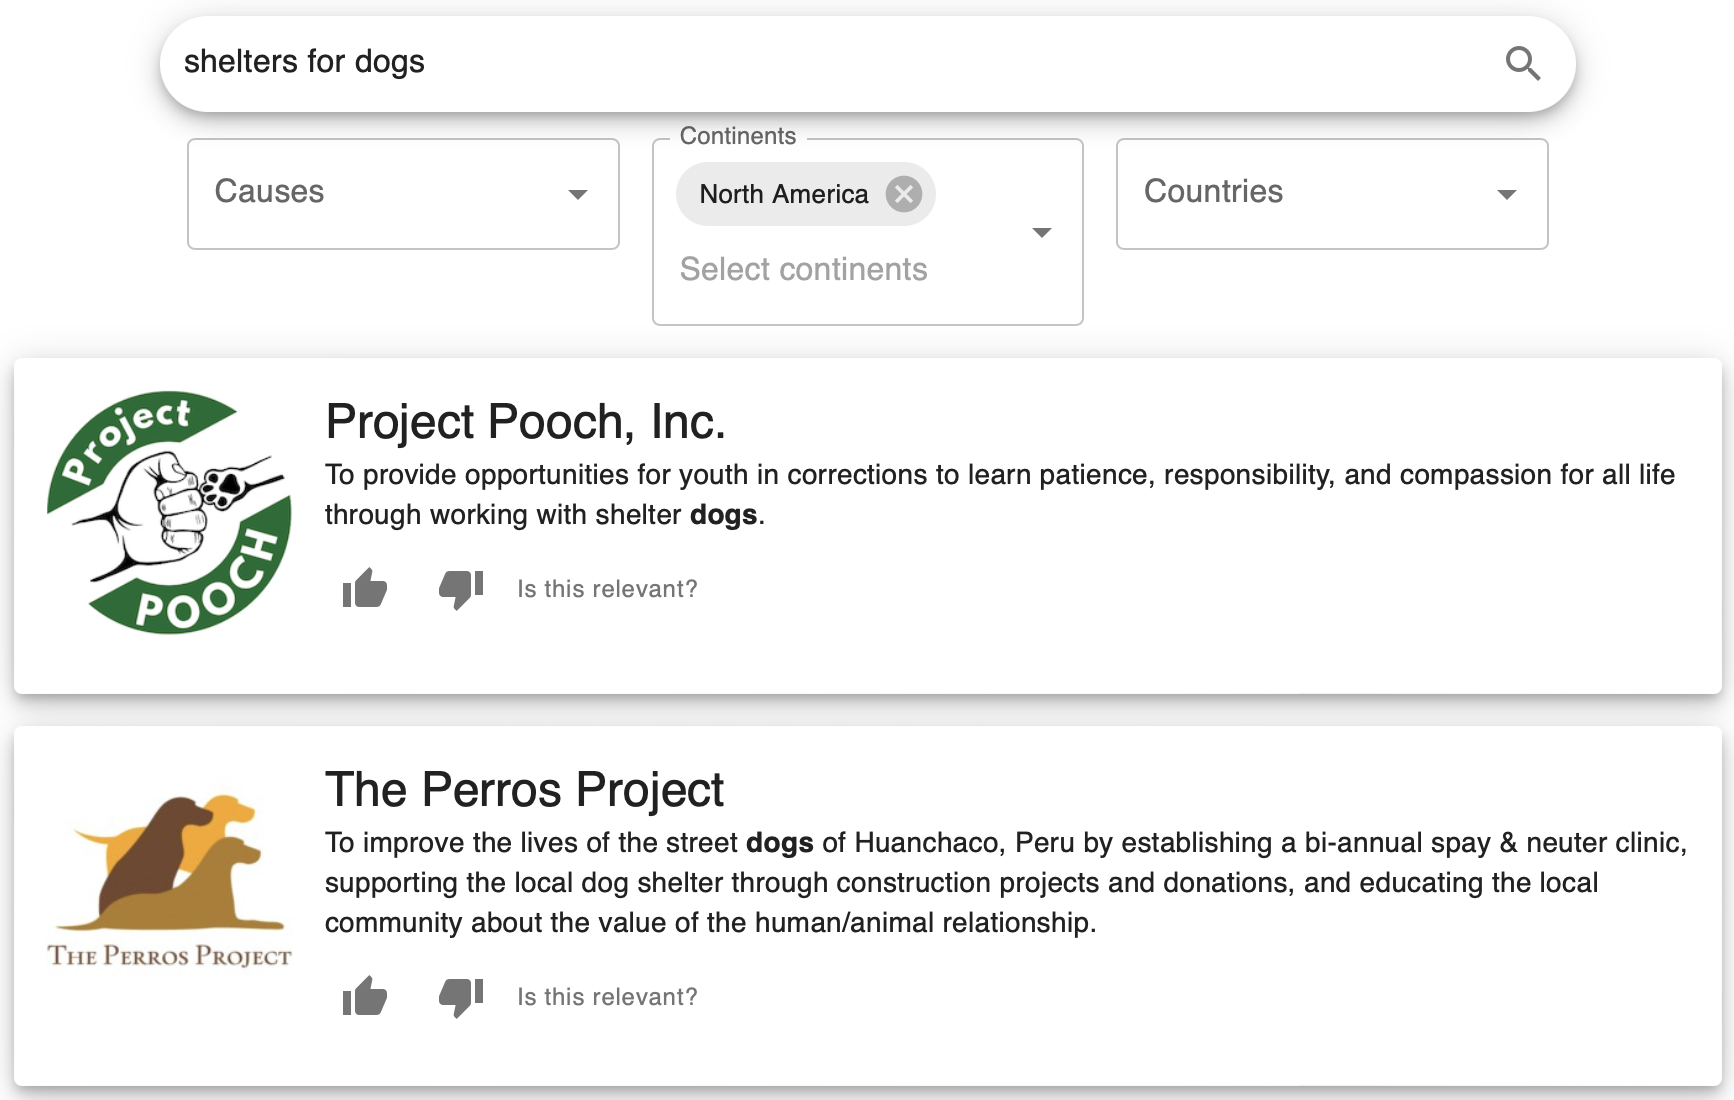
\includegraphics[width=0.6\linewidth]{fig/results-page.png}
    \caption{The results page}
\end{figure}


\subsection{The filters}

The filters are always present under the search bar, and allow the user to select one or more option from the possible values.
Autocompletion is supported when picking an option, to make the filtering experience less time-consuming.
The selected options are shown to the user, allowing to easily see the and remove the filters currently set.
Clicking on the search icon will search results relevant to the query and filter them according to the chosen filters.

As metioned previously, the options of each filter are taken from the actual values that the fields take in all the charities in the data.
We decided to do this so that the user can see what options are available in order to inspire them and give them an overview of what's available.
The list of options is computed in the backend once, and retrieved statically from the frontend as a JSON object.

\begin{figure}[h]
    \centering
    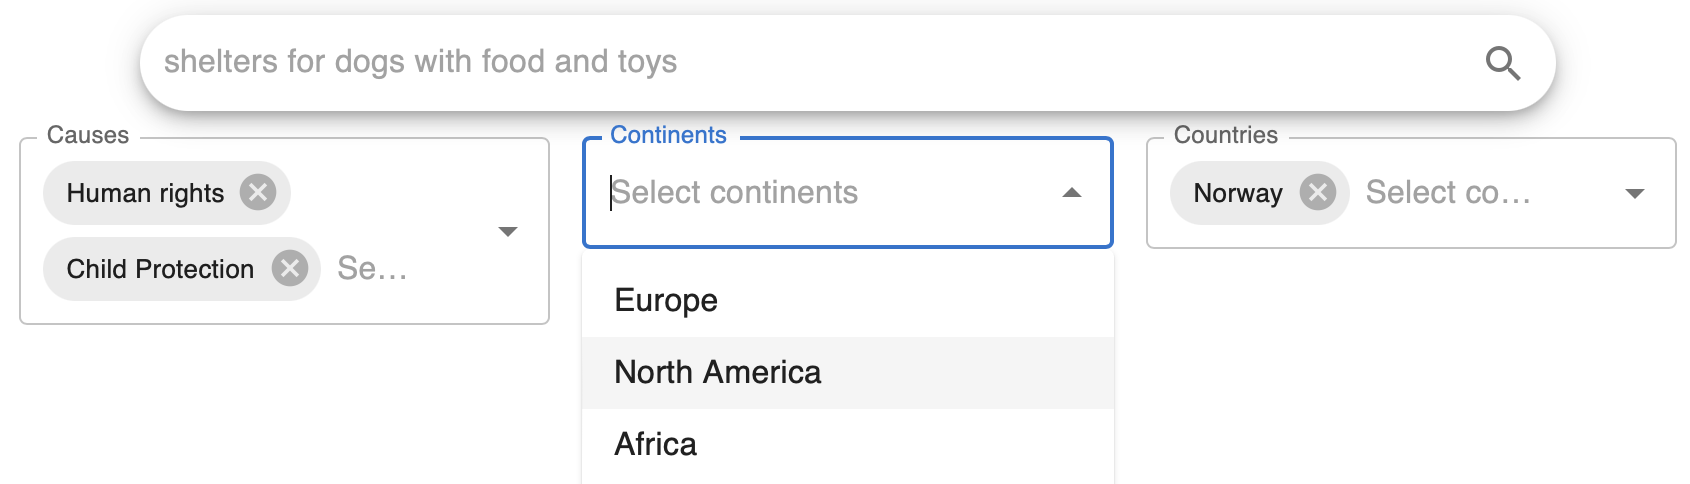
\includegraphics[width=0.6\linewidth]{fig/filters.png}
    \caption{The filters}
\end{figure}

\section{Data Collection and Processing}

We obtained the data from two websites, using a mix of leveraging their API's and applying scraping methods.
The two websites are \href{https://www.globalgiving.org}{Global Giving} and \href{https://www.charitynavigator.org}{Charity Navigator}.

The data has been obtained using the Jupyter Notebooks in the folder \texttt{scraping}. The resulting JSON files have then been moved into the backend to allow static data retrieval when building the index.


\subsection{Global Giving}
Global Giving provides structured data on charitable organizations through its API in XML format. We utilized this API to collect comprehensive information about each charity, ensuring a standardized method of data retrieval.

\subsubsection{Data Retrieval}
To gather data, we accessed the Global Giving API and downloaded XML files containing details of various organizations. The use of their API eliminated the need for web scraping, allowing us to work directly with structured data. The XML files provided the following information about each charity:
\begin{itemize}
    \item Basic details such as the charity's name and location.
    \item Mission statements and website URLs.
    \item Themes representing the causes they work on.
    \item Countries where the organizations operate.
\end{itemize}

\subsubsection{Data Processing}

After retrieving the data, we developed a parser using Python's \texttt{ElementTree} library to extract information from the XML format. To enhance the dataset:
\begin{itemize}
    \item Geographical information was added using \texttt{pycountry} and \texttt{pycountry\_convert}, allowing us to classify organizations by continent based on their headquarters.
    \item Field names were standardized to align with the data structure of Charity Navigator, ensuring consistency across platforms.
    \item The final dataset was converted to JSON format for easier storage and readability.
\end{itemize}

\subsection{Charity Navigator}
Charity Navigator offers data through its GraphQL API. Unlike Global Giving, Charity Navigator does not provide organization logos, requiring additional processing to locate this information.

\subsubsection{Data Retrieval}
Using the GraphQL API, we tailored queries to retrieve:
\begin{itemize}
    \item Organization details, including names and locations.
    \item Causes, mission statements and website URLs.
\end{itemize}
The GraphQL API's flexibility allowed us to avoid redundant data requests and efficiently handle nested data structures. 10,000 records were retrieved in batches of 10 to not flood the server.

\subsubsection{Data Processing}
The lack of logos in Charity Navigator's data required us to develop a custom solution for locating and extracting organization logos from their websites. This system:
\begin{itemize}
    \item Parsed webpage structures using \texttt{BeautifulSoup} to identify elements marked as logos.
    \item Checked metadata and special tags (e.g., \texttt{svg}) for logo information.
    \item Scanned for images commonly used as logos, filtering out irrelevant elements like favicons or menu icons.
\end{itemize}
Standard Python libraries, including \texttt{requests}, \texttt{BeautifulSoup}, and \texttt{re}, facilitated these operations. Finally, the processed data was converted to JSON format to match the structure of Global Giving's dataset.

\section{Backend and Indexing/Retrieval}

\subsection{Indexing and Retrieval}

For the indexing we used Python-Terrier with the Retriever model "BM25".

\subsubsection{The Documents}

The data is collected from the JSON files produced by the scraping, and charities with missing data are removed.
In the index, the "text" column in the Pandas DataFrame for each charity will contain a combination of the charity's name and the charity's mission, so that the user can find results based on both the title and the description.

\subsubsection{The Index}

The index documents are kept in the folder \texttt{backend/index\_docs}, and we used BM25 as the retrieval model. After the query is inserted, and the list of relevant documents is obtained, each document is mapped to its corresponding charity object using the "docno" column, and the ranked list of charities is returned to the frontend.

\subsubsection{The Relevance Feedback}

For the relevance feedback, a dictionary \texttt{feedback} is kept, containing the feedback information for each session. When the user inserts a new query, the session is restored so that the feedback on a previous query doesn't affect the feedback on a new query.
For each session the feedback is kept in the form of a list of  \texttt{(docid, relevant)} pairs.

We perform query augmentation using TF-IDF, considering all the feedback provided on a single query.

The documents on which the user has expressed feedback are separated into relevant documents and non-relevant sets. Using a TF-IDF vectorizer with tokenization and stopword removal, we generated a term-document matrix for both relevant and non-relevant documents.
Then, term weights are computed by summing TF-IDF scores from relevant documents and subtracting scores from non-relevant ones. This emphasizes terms strongly associated with relevant documents while downplaying those linked to non-relevant ones.
Terms are sorted by their computed weights, and positively weighted terms are added to the original query. Original terms are retained to preserve the query's context.

This approach dynamically refines the query by integrating the feedback of the user, enhancing the relevance of the query.



\subsection{The Backend}

Since we used Python-Terrier for the retrieval, we decided to have a backend in Python, and we used Fast API.

The backend contains two routes, one is used for the retrieval based on the query and filters, the other is used for the user relevance feedback.

The retreival of the document and the indexing are performed only once, when the backend is initialized.

\subsubsection{The Routes}

\begin{itemize}
    \item \texttt{GET /search?query=<query>\&session\_id=<session\_id>}: \newline
          This route takes the following parameters:
          \begin{itemize}
              \item \texttt{query}: a string representing the query input by the user
              \item \texttt{session\_id}: the id of the session. A session starts when a new query is inserted, and is used to keep track of the relevance feedback for a specific query.
              \item \texttt{causes}: optional list of strings containing the filtering information of the cause attribute.
              \item \texttt{continents}: optional list of strings containing the filtering information of the continent attribute.
              \item \texttt{countries}: optional list of strings containing the filtering information of the country attribute.
          \end{itemize}
          This route takes the index and the documents initialized when the backend is run, and performs a retreival of the documents relevant to the query. Once the ranked list of results is obtained, it is mapped to a list of charity objects that are then filtered according to the filters specified in the request. The resulting list is returned as a response to the request.
          The result is a list of objects with the following attributes:
          \begin{itemize}
              \item \texttt{score}: the score of the document.
              \item \texttt{docid}: the id of the document in the index.
              \item \texttt{charity}: a complex object containing all the information of the charity, like the name, logo, mission, coutnry, etc\dots .
          \end{itemize}
    \item \texttt{POST /feedback/<session\_id>/<docid>/<relevant>}:\newline
          This route takes the following parameters:
          \begin{itemize}
              \item \texttt{session\_id}: the id of the session.
              \item \texttt{docid}: the id of the document on which the feedback is expressed.
              \item \texttt{relevant}: 1 if the user has identified the document as relevant to the query, 0 otherwise.
          \end{itemize}
          This route adds information about the feedback regarding the session specified. For each session there is a list of feedback entries for each \texttt{(docid, relevant)} pair.
          After the feedback for the session has been updated, the query augmentation is performed using TF-IDF considering ALL the documents that the user has specified as being relevant or not relevant to the query.
\end{itemize}



\section{User Evaluation}

\subsection{Aim of Evaluation}

We want to evaluate the following features:

\begin{itemize}
    \item Usability of User Interface (can the user formulate queries and understand the result page?)
    \item Clarity of Result Snippets (can the user understand the results?)
    \item Relevance of Results (is the user satisfied with the results of the query?)
    \item Filters (can the user figure out how to use filters?)
    \item Relevance Feedback (does the user understand how to give feedback on the relevance of documents?)
\end{itemize}

\subsection{Experimental Hypotheses}

Our hypotheses is that the users will be able to perform a series of tasks in the hypotized number of clicks, and number of queries, without the need of external help.

\subsection{Experimental Methodology}

\subsubsection{The Methodology}

\begin{itemize}
    \item \textbf{Data}: the collection used in the experiment is the total set of charities collected during the scraping.
          The data set is current, since the scraping was performed recently, but this does not have a big influence in the context of charities.
          As we are using the whole data set obtained from the scraping, the data set should be large enough.
    \item \textbf{Experimental subjects}: the experiment will be conducted on 3 subjects taken from people attending the IR course this year. They are not expected to be experts in terms of charities, but they are expected to have familiarity with retrieval systems.
    \item \textbf{Search tasks}: the subjects will be asked to perform 4 given tasks. No help will be given to the subjects unless they raise questions. The need for help will be noted in the experiment. As the users are not expected to be familiar with charities, we do not provide them with real search tasks.
    \item \textbf{Criteria}: The performance of the subjects at each task will be measured in terms of:
          \begin{itemize}
              \item number of clicks
              \item number of queries (when a user clicks on the search button)
              \item whether they needed external help
          \end{itemize}
          The performance of the system at each task will be measured in terms of:
          \begin{itemize}
              \item whether the system raises any unexpected errors
              \item how relevant the results are to the query
          \end{itemize}
          All the criteria are quantitative data, except for the relevance of the results, which is a form of qualitative data and will be measured by the user with a Likert scale
\end{itemize}

\subsubsection{The Tasks}

We selected the following tasks:
\newline

\begin{tabular}{c|c|l}

    Task ID & Feature Tested              & Task                                                             \\ \hline
    T1      & Usability of User Interface & "Find a charity that provides shelters for dogs"                 \\
    T2      & Filters                     & "Narrow results to Africa"                                       \\
    T3      & Clarity of Result Snippets  & "Find out more information about the first result"               \\
    T4      & Relevance Feedback          & "Mark a charity as relevant and review updated recommendations." \\
\end{tabular}

\subsubsection{The Experimental Matrix}

\begin{tabular}{c|c|c|c|c}

    Subject   & First Task & Second Task & Third Task & Last Task \\ \hline
    Subject 1 & T1         & T2          & T3         & T4        \\
    Subject 2 & T1         & T3          & T2         & T4        \\
    Subject 3 & T1         & T2          & T4         & T3        \\
\end{tabular}

\subsection{The Experiment}

Subjects were given a list of tasks on a printed sheet of paper. The subjects had to do the same tasks but in different orders.
Before the start of the experiment, the subjects were informed to only ask for help if they couldn't figure it out on their own, and to signal to the observer when they thought they had completed each task.

This was done because the need of external help is a criteria we are measuring, so each user was aware of the possibility of asking for help, but also incentivized to try to ask as little as possible.

\subsection{The Results}

\subsubsection{The Expected Results}

The following table represents the measurements expected from the users.
\newline

\begin{tabular}{c|c|c|c|c|c}
    Task ID & clicks & queries & need of external help & system raises errors & results are relevant \\ \hline
    T1      & 2      & 1       & no                    & no                   & yes                  \\
    T2      & 3      & 1       & no                    & no                   & yes                  \\
    T3      & 1      & 0       & no                    & no                   & yes                  \\
    T4      & 2      & 0       & no                    & no                   & yes                  \\
\end{tabular}

\subsubsection{Subject 1}

\begin{tabular}{c|c|c|c|c|c}
    Task ID & clicks & queries & need of external help & system raises errors & results are relevant \\ \hline
    T1      & 2      & 1       & no                    & no                   & yes                  \\
    T2      & 3      & 1       & yes                   & no                   & yes                  \\
    T3      & 1      & 0       & no                    & no                   & yes                  \\
    T4      & 2      & 0       & no                    & no                   & yes                  \\
\end{tabular}

\vspace{0.2cm}

\textbf{Note:} The user had issues filtering the results, after seeing that the results were not changing they asked for help to the observer, 
who explained that they needed to click on the search button to apply the filters.

\subsubsection{Subject 2}

\begin{tabular}{c|c|c|c|c|c}
    Task ID & clicks & queries & need of external help & system raises errors & results are relevant \\ \hline
    T1      & 2      & 1       & no                    & no                   & yes                  \\
    T2      & 8      & 1       & yes                   & no                   & yes                  \\
    T3      & 1      & 0       & no                    & no                   & yes                  \\
    T4      & 2      & 0       & no                    & no                   & yes                  \\
\end{tabular}

\vspace{0.2cm}
\textbf{Note:} The user had issues filtering the results, they tried to remove and re-apply the filter after seeing that the results were not changing.
They ended up asking for help to the observer, who explained that they needed to click on the search button to apply the filters.

\subsubsection{Subject 3}

\begin{tabular}{c|c|c|c|c|c}
    Task ID & clicks & queries & need of external help & system raises errors & results are relevant \\ \hline
    T1      & x      & x       & x                     & x                    & x                    \\
    T2      & x      & x       & x                     & x                    & x                    \\
    T3      & x      & x       & x                     & x                    & x                    \\
    T4      & x      & x       & x                     & x                    & x                    \\
\end{tabular}

\subsection{Data Analysis}


\end{document}